\newenvironment{conditions}
  {\par\vspace{\abovedisplayskip}\noindent\begin{tabular}{>{$}l<{$} @{${}={}$} l}}
  {\end{tabular}\par\vspace{\belowdisplayskip}}

In order to deploy the new infrastructure, we first need an estimation of resources that Kubernetes will need in order to handle the same load as the physical infrastructure.
To make this estimation, we have stress tested each Quality of Service (QoS) and monitored the resources consumption. 

\subsection{Service level indicators}

In order to be able to answer each Quality of Service (QoS) differently, we have specified some metrics to help resource optimization without ignoring performance.
The defined metric that will be discussed here and will vary among each QoS is the capability of answering requests per second.

Using the physical infra as starting point (fig. \ref{fig:website_bandwidth}), we can observe the requests per second peaked on the most popular website, with around 16000 requests in an hour which averages on 4.4 requests per second.
We, therefore, have defined that there are three type of websites that translates into three types of Quality of Service:
\begin{itemize}
    \item \textbf{Critical} websites, these are the most popular and therefore the most important to have high capability of requests, the defined value is to handle 35 requests per second (Around 8 times the average on peak usage).
    \item \textbf{Standard} websites, these usually don't face as much traffic and therefore don't need to have high capability of requests, the defined value is to handle 10 requests per second. 
    \item \textbf{Test} websites, as in the name itself, these are used to test new features or add new content by website managers, and therefore are used by testers and developers, these type of websites only need to handle few requests, therefore the defined value is to handle 2 requests per second.
\end{itemize}

%- entire infra: 250 req/sec
%- critical website: 35 req/sec
%- standard website: 5-10 req/sec % TODO set final value
%- test website: 2 max threads

%- Find configuration that is able to handle specified req/sec load
%- Two Graphs (1 for critical and 1 normal), showing AVG response time plots + Request per second plots
%- See the Resources usage for each configuration
%- Make an estimation of total resources , note that critical websites will have $(MAX_LOAD) + 2(IDLE_LOAD)$ since they will have 3 pods

%Total number of Critical websites: 20
%Total number of Standard websites: 600
%Total number of Test websites: 500
%- Make an estimation of total infra resources ( sum to the estimation of total resources with openshift-* elements)

% #### Resources used in the physical infra:
% - Memory: 2TB
% - CPU: 512

\subsection{Stress test setup}

% (we have provioned websites and migrated data from the old infra)
To have a proper setup to test, we have migrated some websites with diversified content to the new infrastructure to observe how websites already hosted under the Physical infra perform on the Kubernetes infrastructure.

%To evaluate the behavior of our Kubernetes infrastructure, with the goal of analysing the new infrastructure's capability of answering the same needs with fewer resources, the following experiment was conducted.

%The following elements were required, 

The experiment has a dedicated Kubernetes cluster that deploys a custom tool based on \hyperlink{locust.io}{Locust} to make multiple requests to the targeted website on the new infrastructure. 
The simulation of requests is done by running multiple \hyperlink{https://kubernetes.io/docs/concepts/workloads/pods/}{Pods}, each containing multiple processes that will request URLs at random\footnote{It iterates urls through the website to discover all the URLs, and only after having all the URLs, it connects to one of them at random}.

\subsubsection{Stress load}
Multiple runs have been made with different configurations in order to find a suitable one for each QoS to process the desired requests per second with minimal resource consumption.

We observed that after a number of parallel users in the same pod, the users would get bottle-necked by Pod network constraints. So for our tests we observer that each Pod could have no more than 5 processes before network constraints would interfere.

%Important notes:
%- RAM consumption before first connection is ~11MiB, 500 to 600MiB after (even if no accesses are being done)
%- Time used for a stress run was decided to be 6min because it's enough to see the stabilized response time

\subsubsection{Measurements}

The following graph shows the average response time from the client's side as well the requests per second handled from the server side at the same time. 

The stress tests do a ramp up during the first minute, after which they maintain the stress load for more 9 minutes.
Thus, the total duration for each run is 10minutes, this value was considered enough to present the trend that would follow in a bigger time frame.

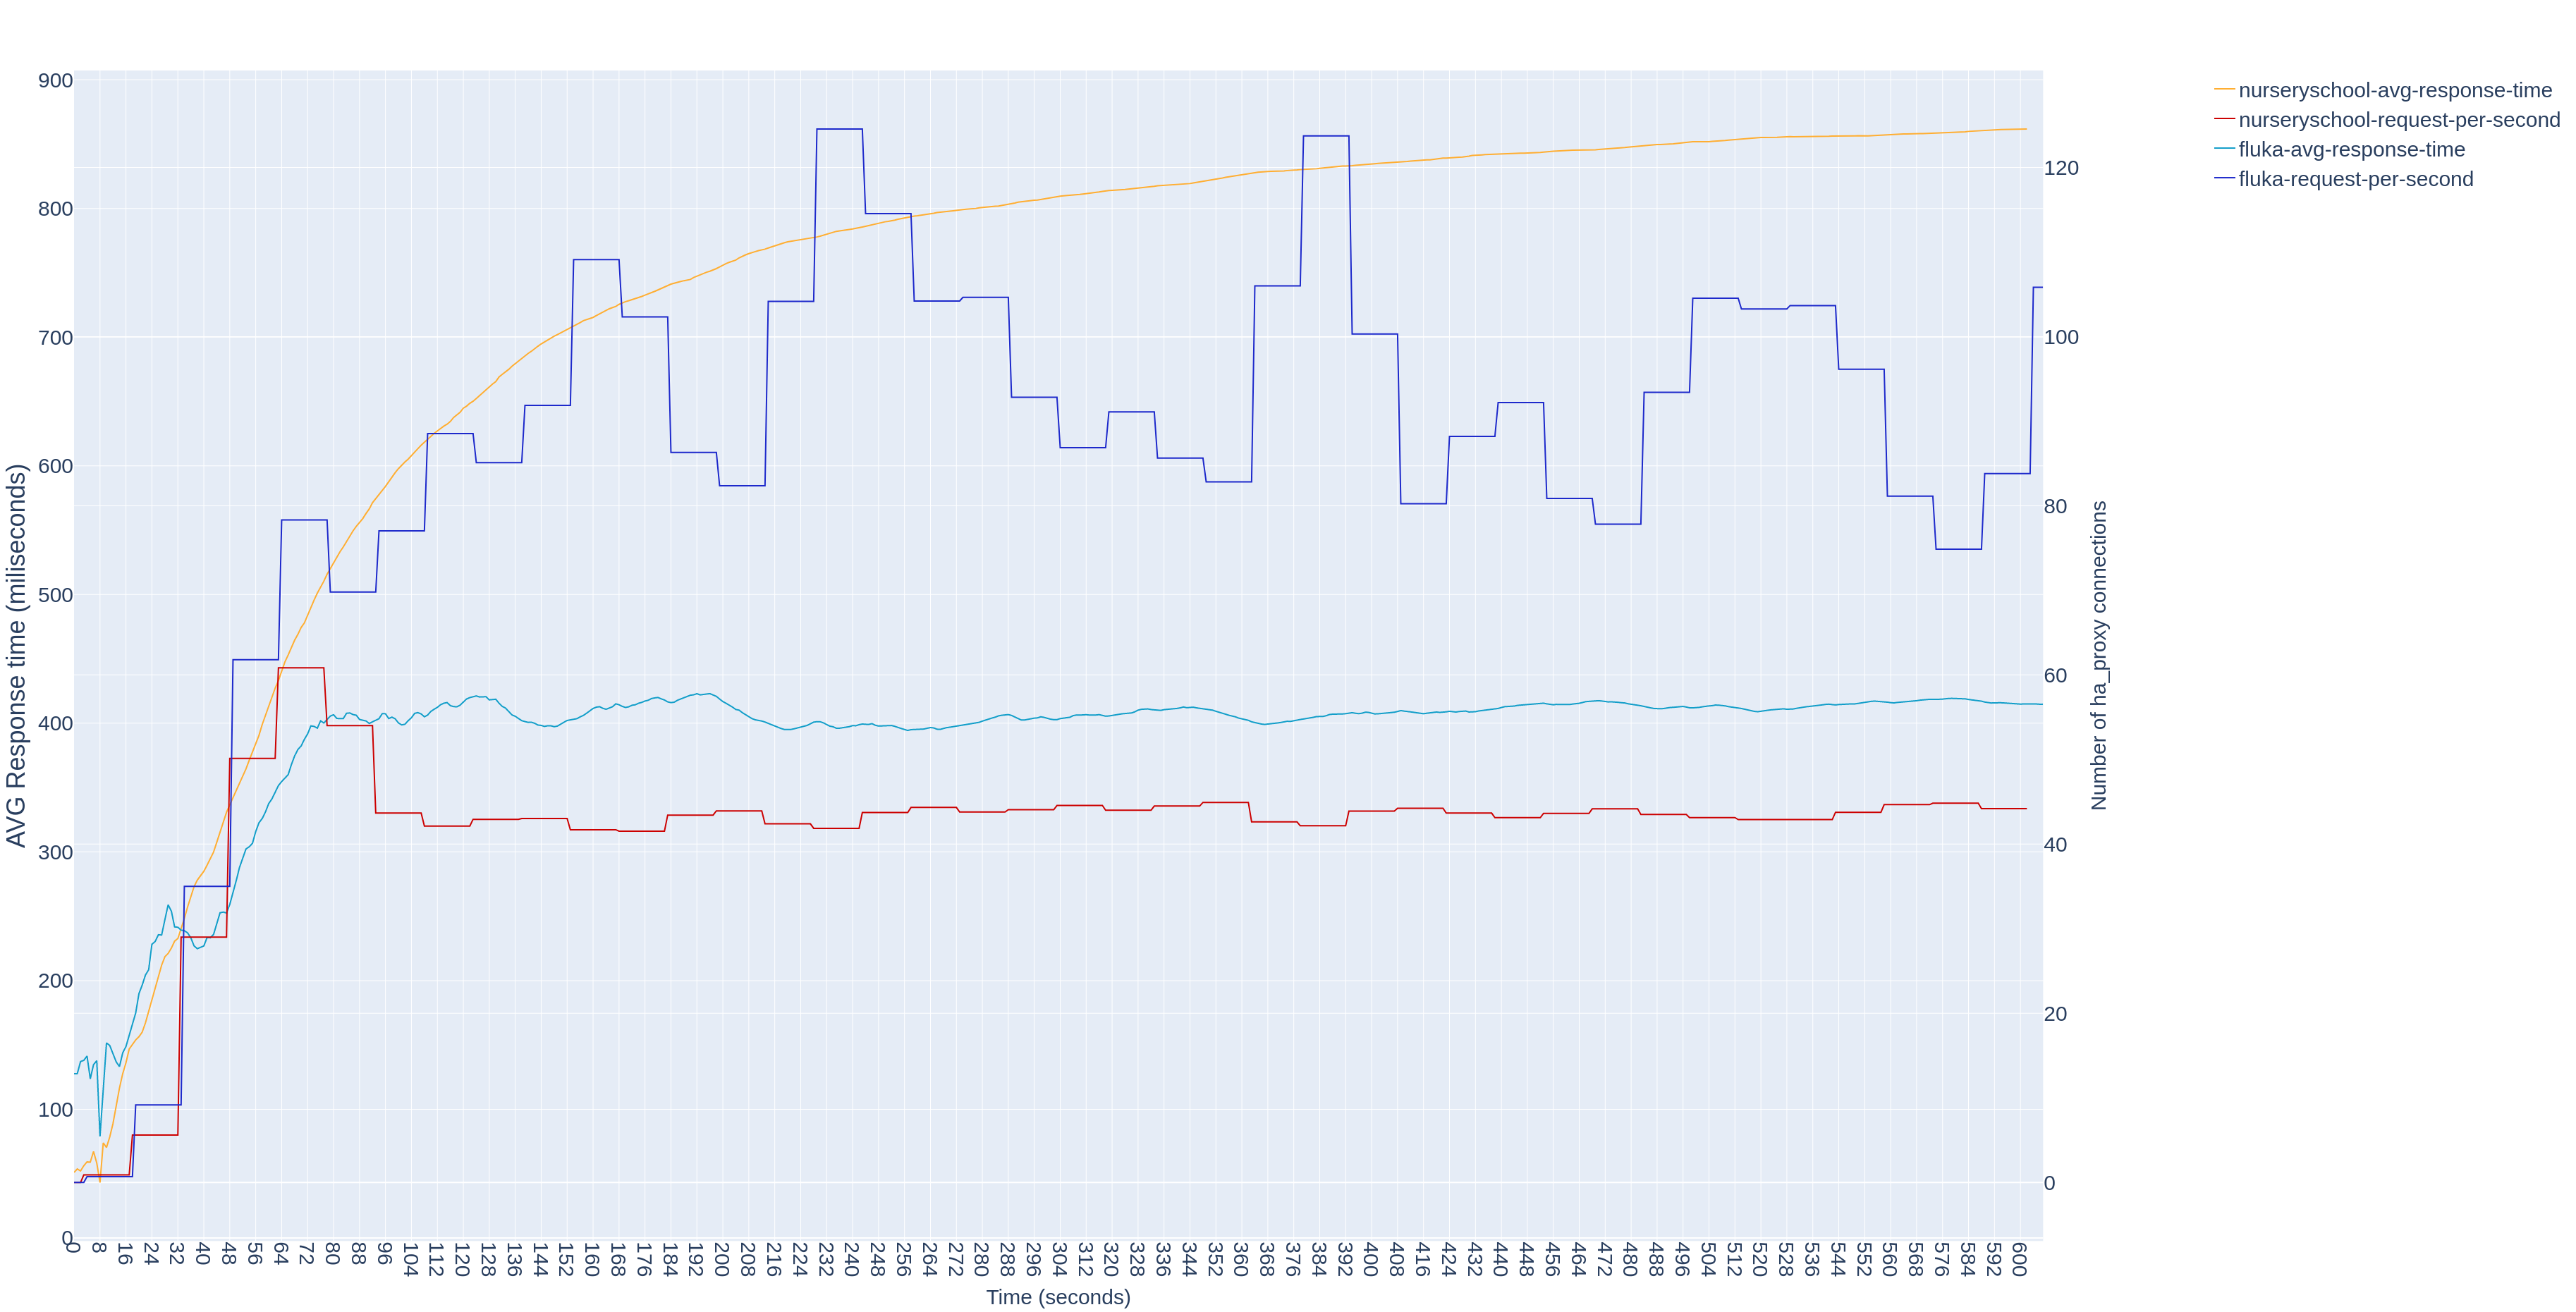
\includegraphics[width=400]{figures/experiment-figures/critical_run.png}

During this run, the resources consumption was also monitored, here we can see the usage for `nursery` and `fluka` websites respectively:

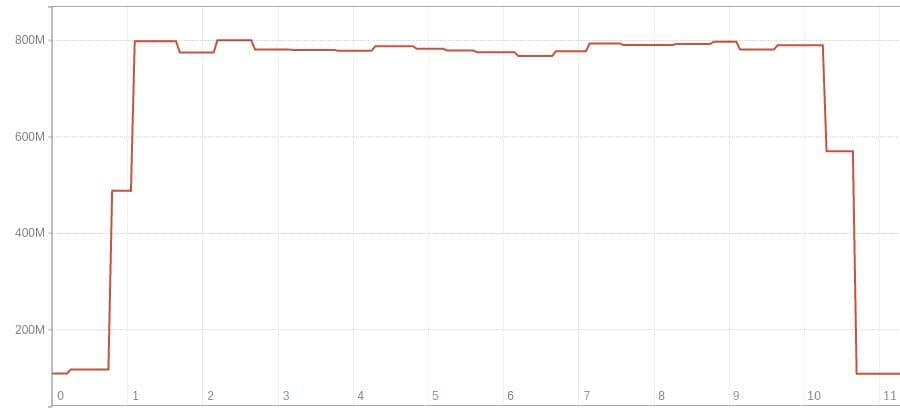
\includegraphics[width=\linewidth/2]{figures/experiment-figures/nursery_memory_usage.jpg}
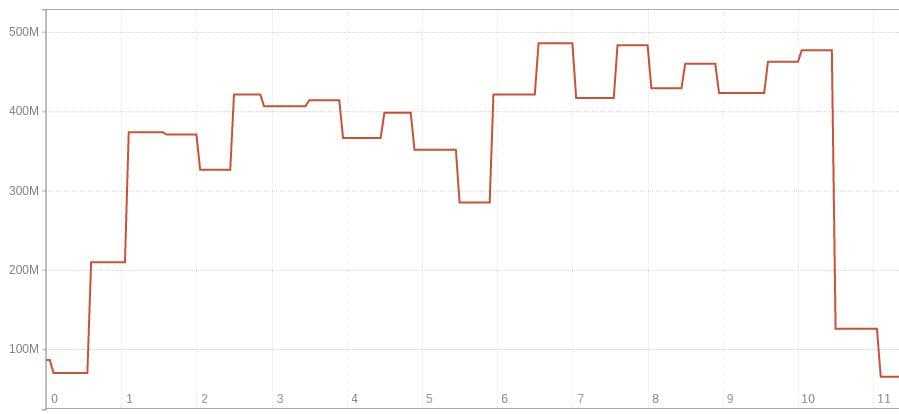
\includegraphics[width=\linewidth/2]{figures/experiment-figures/fluka_memory_usage.jpg}

The same experiment was conducted to the same websites with configurations based on the other QoS. 
The following tables show the highest response time under full stress and lowest requests per second for each QoS.

\begin{table}[!htb]
\centering

\begin{tabular}{|l|ll|ll}
\cline{1-3}
\textbf{website} & \multicolumn{1}{l|}{\textbf{Stress (req/s)}} & \textbf{Response (ms)} &  &  \\ \cline{1-3}
nurseryschool    & 10                                           & 510                    &  &  \\ \cline{1-1}
fluka            & 26                                           & 570                    &  &  \\ \cline{1-3}
\end{tabular}
\caption{Test QoS Values}


\begin{tabular}{|l|ll|ll}
\cline{1-3}
\textbf{website} & \multicolumn{1}{l|}{\textbf{Stress (req/s)}} & \textbf{Response (ms)} &  &  \\ \cline{1-3}
nurseryschool    & 18                                           & 240                    &  &  \\ \cline{1-1}
fluka            & 48                                           & 103                    &  &  \\ \cline{1-3}
\end{tabular}
\hfill
\caption{Standard QoS values}
\begin{tabular}{|l|ll|ll}
\cline{1-3}
\textbf{website} & \multicolumn{1}{l|}{\textbf{Stress (req/s)}} & \textbf{Response (ms)} &  &  \\ \cline{1-3}
nurseryschool    & 41  & 870   &  &  \\ \cline{1-1}
fluka            & 74  & 600   &  &  \\ \cline{1-3}
\end{tabular}
\caption{Critical QoS values}
\end{table}


%Table \ref{tabel_of_resources}
\begin{table}[]
\centering
\label{tabel_of_resources}
\begin{tabular}{|l|ll|ll}
\cline{1-3}
\textbf{QoS} & \multicolumn{1}{l|}{\textbf{CPU}} & \textbf{RAM(MiB)} &  &  \\ \cline{1-3}
test         & 0.3                                & 104               &  &  \\ \cline{1-1}
standard     & 2.3                                & 257               &  &  \\ \cline{1-1}
critical     & 3  & 800               &  &  \\ \cline{1-3}
\end{tabular}
\caption{ Resources peak consumption per QoS.}
\end{table}
% Show that we have STABLE response times

\subsection{Results: resource provision}

Based on the results seen in measurements section, we can now make an estimation of resource provision for the new infrastructure based on the values retrieved.

For expected memory:
\[
\begin{array}{rcl}
TotalMem & = & C * L + 2* C * I + S * L + T * L \\
 & = & 20 * 960MiB + 20*104MiB + 600*309MiB + 500*125MiB \\
 & = & 269180MiB  \approx  282.3GB
\end{array}
\]
Where:
\begin{conditions}
Expected Load  &  Max Seen load + 20\% overhead \\
 L     &  Expected Max Load for specific QoS website \\
 I     &  Expected Idle Load for specific QoS website \\   
 C     &  Total number of Critical Websites \\
 S     & Total number of Standard Websites \\
 T     & Total number of Test Websites \\
\end{conditions}

On the physical infrastructure we have provisioned 2TB of memory, on the new Kubernetes infrastructure we have a rough estimation on total memory used if all websites are under load is of about 283GB. The prediction expects to only have 14.15\% of the memory required in the physical infrastructure.


For expected cpu:
\[
\begin{array}{rcl}
TotalCPU & = & C * L + 2* C * I + S * L + T * L \\
 & = & 20 * 3VCpu + 2*0.01VCpu + 600* 1.6VCpu + 500* 1VCpu \\
 & = & FINALRESULT
\end{array}
\]


